%%
%% 研究報告用スイッチ
%% [techrep]
%%
%% 欧文表記無しのスイッチ(etitle,jkeyword,eabstract,ekeywordは任意)
%% [noauthor]
%%

\documentclass[submit,techrep]{ipsj}
%\documentclass[submit,techrep,noauthor]{ipsj}



\usepackage[dvipdfmx]{graphicx}
\usepackage{latexsym}

\def\Underline{\setbox0\hbox\bgroup\let\\\endUnderline}
\def\endUnderline{\vphantom{y}\egroup\smash{\underline{\box0}}\\}
\def\|{\verb|}

\setcounter{巻数}{53}%vol53=2012
\setcounter{号数}{10}
\setcounter{page}{1}


\begin{document}


\title{データベース及び演習\\
(2023年7月31日)}

\etitle{Database and Exercises \\ (version 2012/10/12)}

\affiliate{IPSJ}{情報処理学会\\
IPSJ, Chiyoda, Tokyo 101--0062, Japan}


\paffiliate{JU}{情報処理大学\\
Johoshori Uniersity}

\author{水谷祐生}{Yusei Mizutani}{IPSJ}[joho.taro@ipsj.or.jp]

\begin{abstract}
本稿は,情報処理学会論文誌ジャーナルに投稿する原稿を執筆する際,および論
文採択後に最終原稿を準備する際の注意点等をまとめたものである.大きく分け
ると,論文投稿の流れと,\LaTeX と専用のスタイルファイルを用いた場合の論
文フォーマットに関する指針,および論文の内容に関してするべきこと,するべ
きでないことをまとめたべからずチェックリストからなる.本稿自体も \LaTeX 
と専用のスタイルファイルを用いて執筆されているため,論文執筆の際に参考に
なれば幸いである.
\end{abstract}

%
%\begin{jkeyword}
%情報処理学会論文誌ジャーナル,\LaTeX,スタイルファイル,べからず集
%\end{jkeyword}
%
%\begin{eabstract}
%This document is a guide to prepare a draft for submitting to IPSJ
%Journal, and the final camera-ready manuscript of a paper to appear in
%IPSJ Journal, using {\LaTeX} and special style files.  Since this
%document itself is produced with the style files, it will help you to
%refer its source file which is distributed with the style files.
%\end{eabstract}
%
%\begin{ekeyword}
%IPSJ Journal, \LaTeX, style files, ``Dos and Dont's'' list
%\end{ekeyword}

\maketitle

%1
\section{機能概要}
このアプリケーションには
\begin{itemize}
  \item 「作成者名」「部屋名」「部屋の説明」を入力した後、「作成」ボタンを押すことで部屋を作成する機能
  \item 部屋の説明欄を編集する機能
  \item  タグを作成する機能
  \item 作成したタグを部屋の参加者に割り当てる機能
  \item 参加者を追加する機能
  \item 参加者を削除する機能
  \item 参加者カードの「編集」を押すことで「名前」または「コメント」を編集する機能
  \item 部屋の参加者の受付をするかしないかを決める機能
  \end{itemize}
  といった機能が実装されている.

\section{利用技術}
\subsection{Next.js}
\subsubsection{Next.jsとは}
Next.jsとはReactをベースに開発された、フロントエンドフレームワークである.

Next.jsでは画像・レンダリングを最適化する。最適化するメリットとしてページの読み込み速度が高速になることである.また、読み込み速度の高速化はSEOにも効果がある.このようにNext.jsを利用することで、Webページ閲覧時のユーザー体験を向上させる、作成したページを誰かに見てもらいやすくなるといったメリットがある.

\subsubsection{Reactとは}
ReactとはFacebook社が開発したWebサイト上のUIパーツを構築するためのJavaScriptライブラリである.また、JSX記法と呼ばれる構文が採用されていて、これにより一つのファイル内でHTMLタグに対する動きを操作することができる.
同様のJavaScriptのライブラリとしてVue.js、Angularなどが挙げらるが、Reactは中でも世界的に圧倒的な導入率を誇ってている。
\subsection{ChakraUI}
Chakra UIとは、UIコンポーネントライブラリの1つで、自前でCSSを書かなくてもパラメータ指定でスタイルを記述でき、デザインに一貫性を持たせることができる。
再利用可能なコンポーネントも多く用意されていて、アラートダイアログやドロワーメニュー、トーストなど自前で作ろうとすると大変なものも簡単に実現できる。また、レスポンシブ対応も容易に行うことができるため誰でも簡単に洗練されたデザインのUIを構築することが可能である.

\subsection{TypeScript}
TypeScriptとはオープンソースかつ、JavaScriptを拡張して開発されたプログラミング言語であり、Microsoftによって開発された.

基本的な文法はJavaScriptと大した変化はないが、大きな違いとして型付けができるかどうかが挙げられる.

従来までのJavaScriptには型付けがない、つまり動的型付けといって実行時にプログラム側が勝手に数値型、文字型を判定するため実行時のエラーの存在に気づかず思わぬバグに繋がることがあった.この問題を解決するためTypeScriptでは静的型付けといって実行前にプログラマーがあらかじめ型を設定できるようにした.また静的型付けによって、変数の説明ができるため大規模な開発においてソースコードの可読性という観点からも恩恵を受けることができる.


\subsection{Go}
\subsubsection{Go言語とは}
Go言語とは、シンプルかつ高速な処理が可能なプログラミング言語であり、Google社によって開発された.
コードをシンプルかつにそして高速に動作させるというコンセプトの元に開発されたため、他の言語には実装されている機能、例えば「継承」や「ジェネリクス」などが実装されていない.そのため、誰が書いても似たようなコードになり、アプリケーションの管理を簡単にすることができる.
\subsubsection{Ginとは}
GinとはGo言語の中でも人気のあるWebフレームワークである.

Ginには高速なパフォーマンス、JSONのリクエストのバリデーション、ルーティングのグループ化、エラー管理、組み込みのレンダリング、といった特徴があるため、Ginなしで開発するよりもより高速、簡単にWebアプリケーションやAPIサーバーを開発することができる.

\subsection{Docker}
Dockerとは、Docker社が開発するコンテナ型のアプリケーション実行環境のことである.Dockerを使うことで、1台のサーバー上で様々なアプリケーションを手軽に仮想化・実行できるようになる.

Dockerはコンテナ環境をファイルで設定することができるため、Dockerファイルを共有することで開発環境を揃えることが大変であるチーム開発時に大きな有用性がある.また、一台のサーバーに複数のアプリケーション実行環境を作成することができるため、デプロイのしやすさや、サーバーの節約にも貢献することができる.

\subsubsection{API}
APIとは「Application Programming Interface」の略である.言葉通りに意味を解釈すると、アプリケーションをプログラミングするためのインターフェースという意味である.簡単に説明すると、APIとはソフトウェアにAPIという外部とやりとりする窓口であり、外部アプリとコミュニケーションや連携ができるものである.

\section{システム設計}

\subsection{システム概要}
今回のアプリのシステム構成図は図1のようになっており、UI描写専用のNext.jsのサーバーとMySQLサーバーとやり取りを行うGoサーバー今回はフレームワークとしてGinを使用しているためGinサーバーの二つが連携することによって動作するようになっている.具体的な連携方法として、HTTPメソッドでやり取りをを行っており、今回はNext.jsサーバーがGET、POST、PUT、DELETEメソッドにパラメーターやボディーに変数を乗せてGinサーバーにリクエストを送り、バックエンド側でそれに応じたデータベースに対する操作を行い、最終的な結果をNext.jsサーバー、つまりフロントエンドにレスポンスとして返している.

\begin{figure}[htbp]
  \centering
 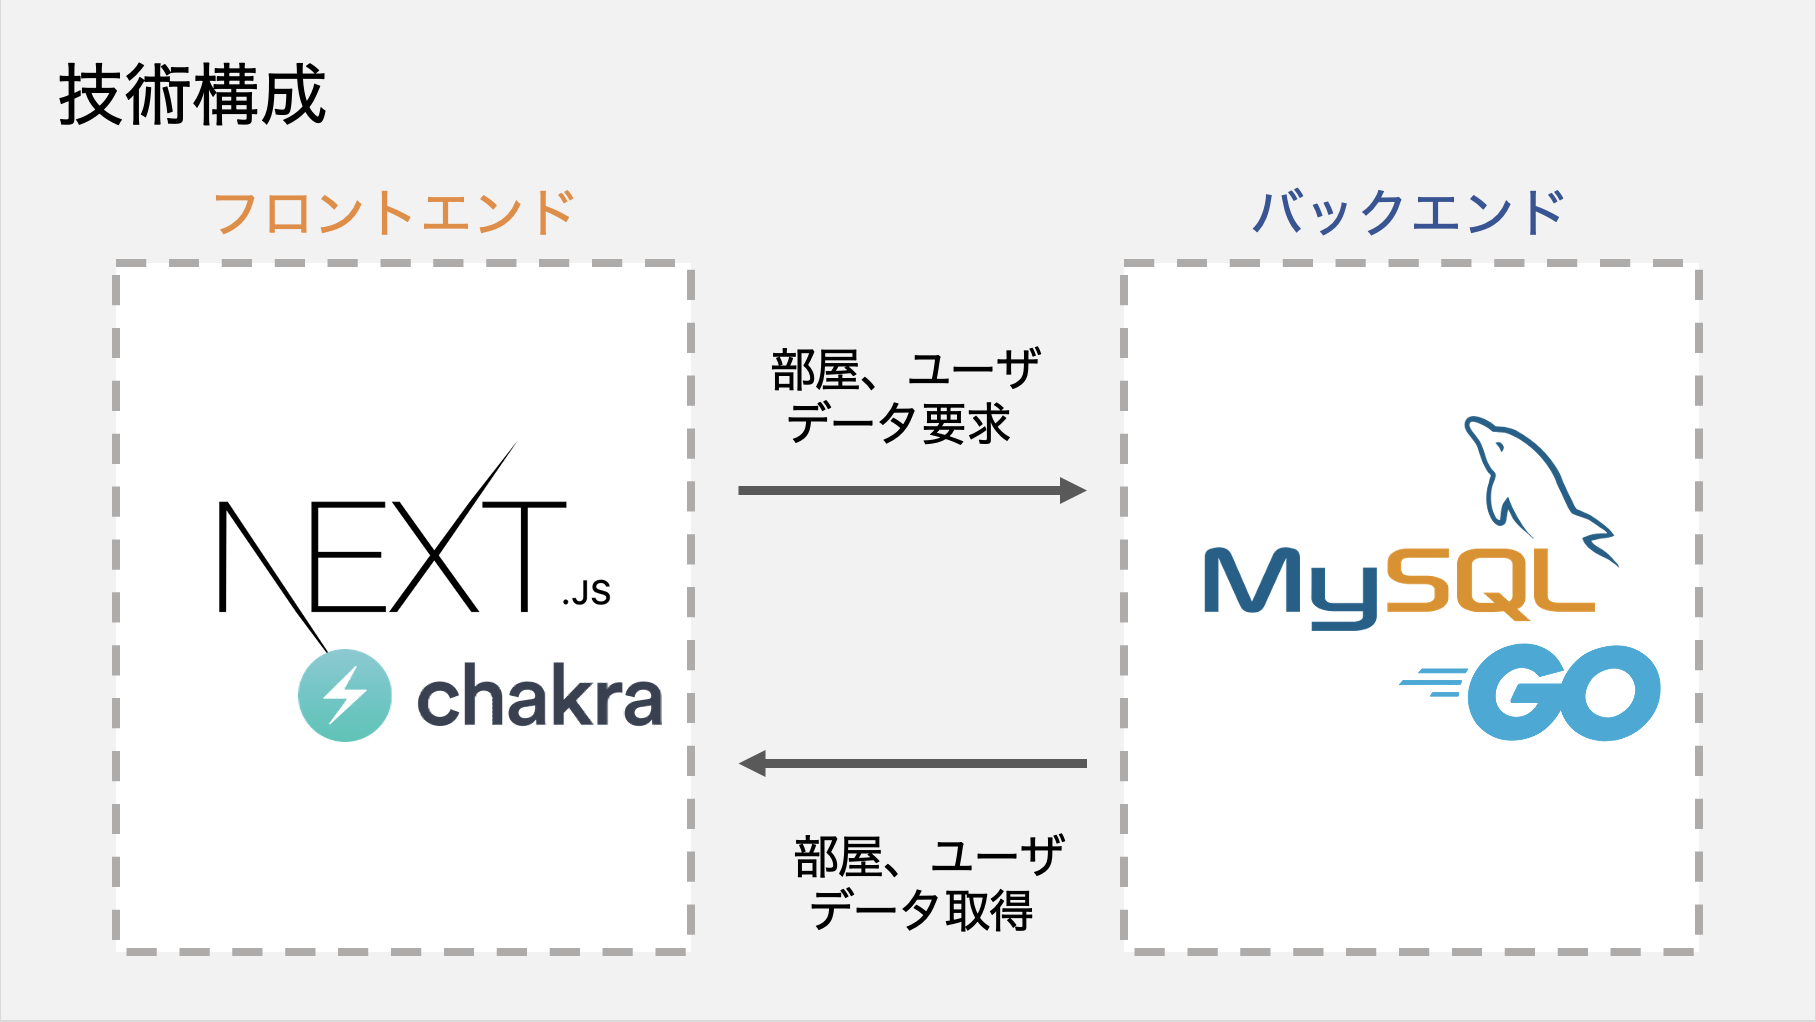
\includegraphics[width=8cm]{./images/technical_configuration.jpg}
  \caption{システム構成図}
  \label{fig:sample}
\end{figure}

\subsection{技術選定の意図}
\subsubsection{Next.js}
Next.jsはデフォルトでサーバーを持っているため、create react appを利用して開発した際に設定しなくてはならないWebpackやbabelの記述の負担を減らすことができるため採用した.

\subsubsection{ChakraUI}
ChakraUIはCSSを記述しなくとも洗練されたデザインのUIコンポーネントを扱うことができるため、フロントエンド側でのデータ処理やクリック時の処理に時間を咲くことができる.すなわち、システム的な機能実装に集中することができるため採用した.

\subsubsection{Go}
他にもPython、Javaなどが候補に上がったが、中でもGo言語はGormといったORMマッパーや、Ginといった強力なWebフレームワークが備わっているため、APIサーバーを作成するために便利なパッケージが備わっている.それゆえに、Go言語を採用した

\subsubsection{MySQL}
今回のアプリの性質上、RDBを用いると最も容易にデータ管理を行うことができると考えたため採用した.



\subsection{画面遷移}

\begin{figure}[htbp]
  \centering
 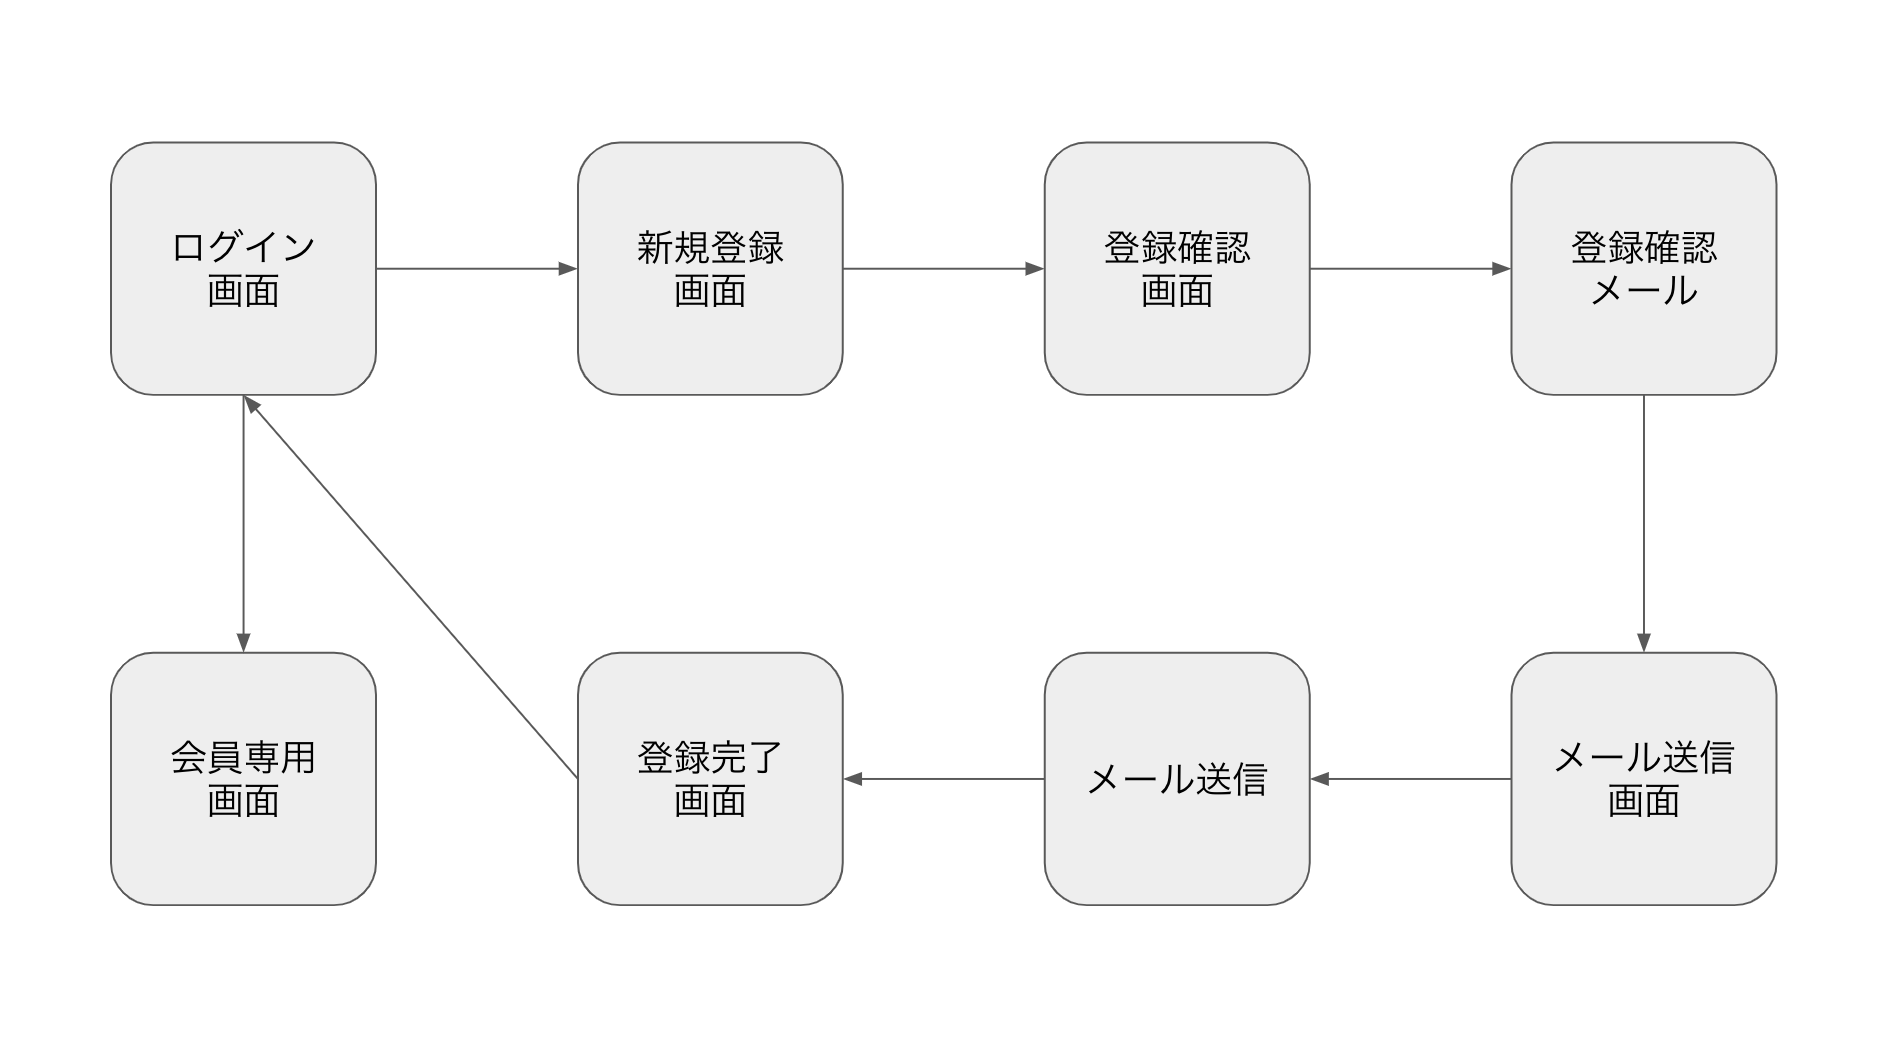
\includegraphics[width=8cm]{./images/screen_transition.jpg}
  \caption{画面遷移の図}
  \label{fig:sample}
\end{figure}

\begin{figure}[htbp]
  \centering
 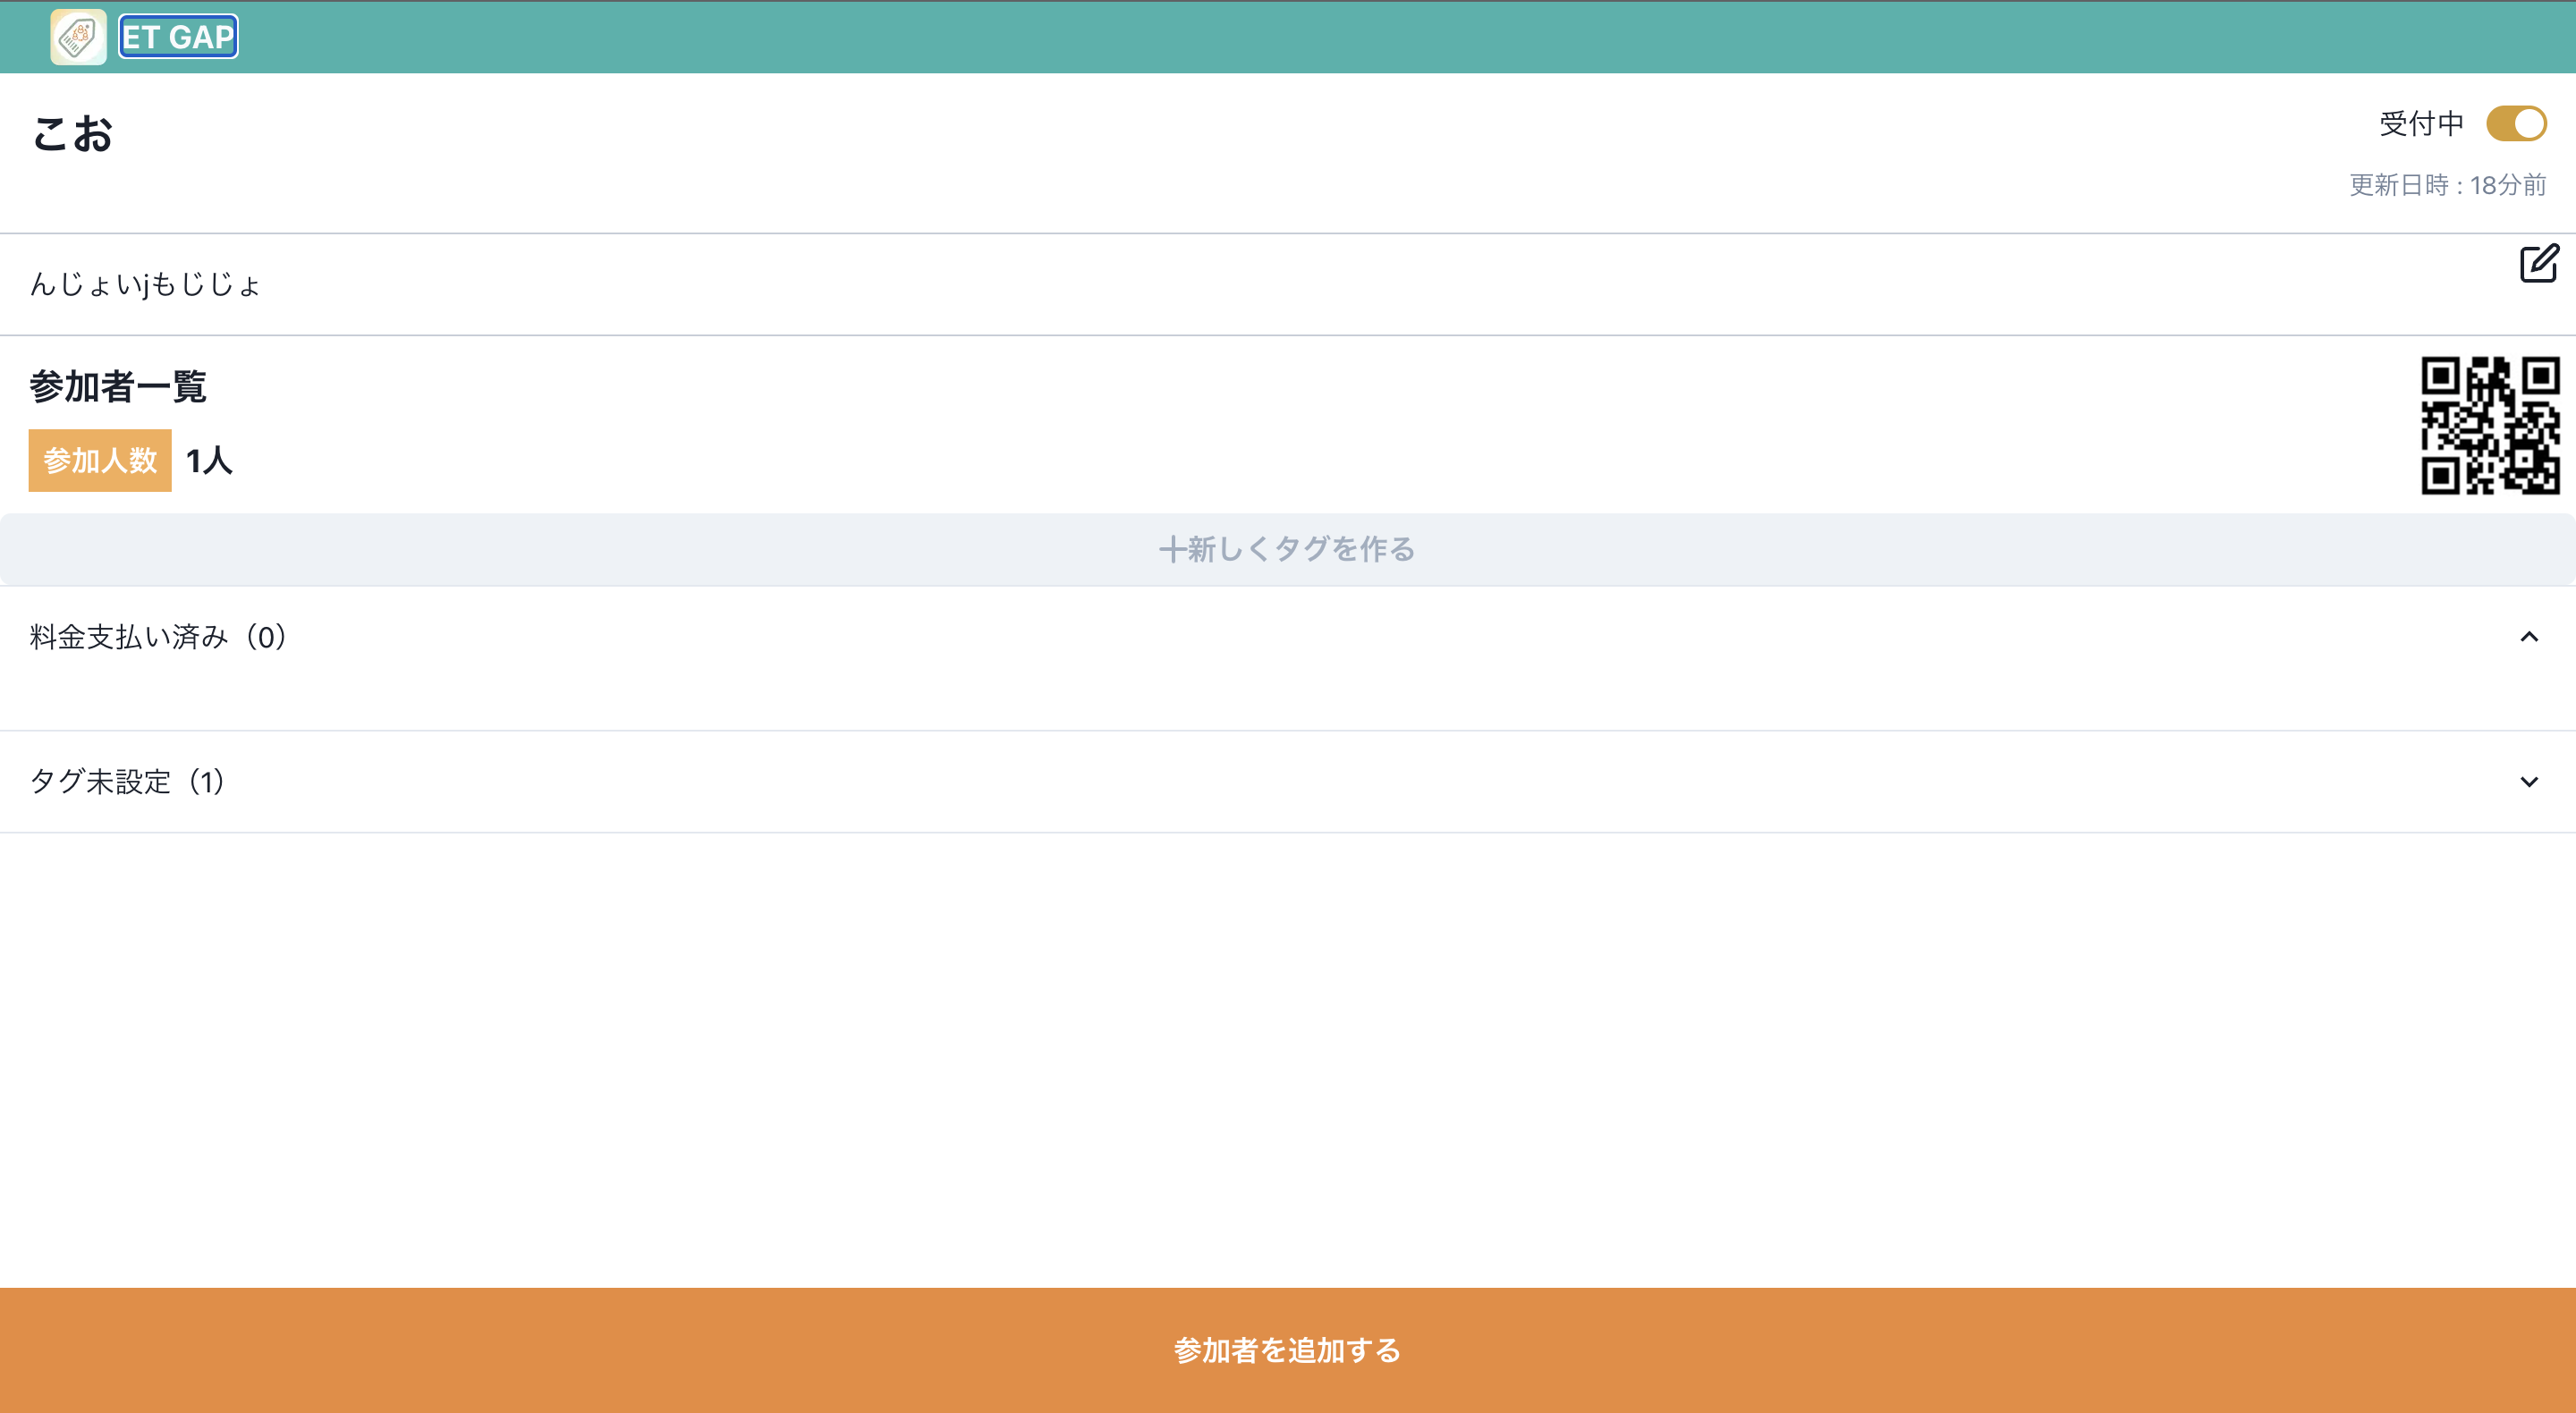
\includegraphics[width=8cm]{./images/room_screen.jpg}
  \caption{部屋画面の図}
  \label{fig:sample}
\end{figure}


図2は今回のプログラムにおける画面遷移を表したものであり、以下にその詳細を記す.
\subsubsection{部屋作成の動き}
\begin{enumerate}
  \item 「部屋一覧画面」で「新しく部屋を作る」ボタンをおして「部屋追加画面」に遷移する
  \item 「部屋追加画面」で作成者名、部屋名、部屋の説明を入力して「作成」ボタンをおす
  \item  ボタンを押したと同時に部屋を新規作成、部屋画面に遷移する
 \end{enumerate}
といった流れになっている.

\subsubsection{部屋参加の動き}
\begin{enumerate}
  \item 部屋に入っている人から「部屋画面」に表示されているQRコードまたはURLを共有してもらう
  \item 「部屋画面」の「参加者を追加する」ボタンを押すと、ドロワーが表示される
  \item  ドロワーにある名前、コメントを入力してから「参加する」ボタンを押す
 \end{enumerate}
といった流れになっている.

\subsubsection{タグ付の動き}
\begin{enumerate}
  \item 「新しくタグを作る」を押す
  \item ドロワーが表示される
  \item ドロワーの「タグ」に作成したいタグ名をつける
  \item 図3のユーザーカードにある「編集」ボタンを押す
  \item 押すと「名前」、「コメント」、「タグ」の入力ができるため「タグ」の欄に作成したタグ名を入れる
 \end{enumerate}
といった流れになっている.

\subsubsection{参加者削除の動き}
\begin{enumerate}
  \item 図3のユーザーカードにある「削除」ボタンを押す
  \item 確認用のドロワーが表示される
  \item ドロワーにある「はい」ボタンをクリックする
 \end{enumerate}
といった流れになっている.

\subsection{Docker内の処理}
今回のアプリケーションはバックエンドを全てDockerで行なっている.このセクションではGoとMySQLコンテナについて、docker-compose.ymlとDockerfileを参照しながら説明をする
\subsubsection{Goコンテナ}
\begin{verbatim}
  go:
    container_name: Database_And_Exercises_Go
    build:
      context: ./Docker/go
      dockerfile: Dockerfile
    stdin_open: true
    tty: true
    env_file:
      - ./Docker/go/.env
    volumes:
      - ./go:/go/src/app
    ports:
      - 8080:8080
    depends_on:
      - "mysql"
\end{verbatim}
上はdocker-compose.ymlの中でもGoコンテナに関する記述を抜粋したものである.
以下、それぞれの部分に関する説明を行う.
\begin{enumerate}
  \item container\_nameでコンテナの名前を指定する.今回は「Database\_And\_Exercises\_Go」
  \item buildのcontextにDockerfileのあるパスをdocker-compose.ymlから見たときのパスを入力し、docekrfileに読み込むDockerfileのファイル名を指定する
  \item  stdin\_openとはコンテナ内のエラーを標準出力として表示するかをbooleanで指定する要素である
  \item ttyとは擬似端末(キーボードによる入力)をコンテナに結びつける設定である
  \item  env\_fileで環境変数として読み込むenvファイルのパスを指定している
  \item volumesで「:」よりも右にあるパス以下のファイル、フォルダを「:」よりも左にあるパス以下に全てコピーする
  \item  ports
  でGinサーバーのポート番号を指定する.今回は8080番を指定した
  \item MySQLコンテナよりも早くGoコンテナが立ち上がっていると実行時にDBに接続ができなくエラーが発生するためdepends\_onでMySQLコンテナが立ち上がってからGoコンテナを立ち上げるようにする
 \end{enumerate}
 

 \begin{verbatim}
FROM golang:1.19.3-alpine
RUN apk add --update &&  apk add git
RUN mkdir /go/src/app
WORKDIR /go/src/app
ADD . /go/src/app
CMD ["go", "run", "./cmd/main.go"]
 \end{verbatim}
上のコードはGoコンテナに関するDockerfileである.
以下、それぞれの部分に関する説明を行う.
\begin{enumerate}
  \item FROM以下に取得したいDockerイメージを取得する.今回はGo言語に関するイメージを取得する
  \item RUNコマンドでビルド時に実行したいコマンドを指定する.今回はgitのインストールとディレクトリを作成した
  \item  WOEKDIRでコンテナに入って操作するとき、一番最初に指定するパスを指定する
  \item ADDでコンテナに指定したフォルダやファイルをコピーする
  \item  env\_fileで環境変数として読み込むenvファイルのパスを指定している
  \item CMDでコンテナを立ち上げたときに実行するコマンドを指定する.今回はコンテナ起動時にGinサーバーを起動させたいため、main.goを実行するようにしている
 \end{enumerate}


\subsubsection{MySQLコンテナ}
\begin{verbatim}
  mysql:
    container_name: Database_And_Exercises_DB
    build:
      context: ./Docker/mysql
      dockerfile: Dockerfile
    ports:
      - "3306:3306"
    volumes:
      - ./Docker/mysql/init:/docker-entrypoint-initdb.d
    environment:
      MYSQL_ROOT_PASSWORD: admin
\end{verbatim}

\begin{enumerate}
  \item container\_nameでコンテナの名前を指定する.今回は「Database\_And\_Exercises\_DB」
  \item buildのcontextにDockerfileのあるパスをdocker-compose.ymlから見たときのパスを入力し、docekrfileに読み込むDockerfileのファイル名を指定する
   \item  portsでMySQLサーバーのポート番号を指定する.今回は3306番を指定した
  \item volumesではMySQLに初期化用のsqlファイルのパスを指定して、それを元にコンテナ立ち上げ時、データベースとテーブルを作成するようにしている
  \item environmentでMySQLコンテナ内のルートパスワードを設定している
 \end{enumerate}

\begin{verbatim}
FROM mysql:latest
COPY mysqld_charset.cnf /etc/mysql/conf.d/mysql_charset.cnf
\end{verbatim}
上のコードはMySQLコンテナのDockerfileである.

以下、それぞれの部分に関する説明を行う.

\begin{enumerate}
  \item FROMはGoコンテナ同様、インストールするイメージを指定している.
  \item COPYでインストールしたイメージにローカルのファイルをコピーしている.今回はMySQLを日本語対応させるためのカセットをコピーしている
 \end{enumerate}


\subsection{データベース設計}
今回作成したアプリケーションでは二つのテーブルが存在する.
一つ目は、部屋情報を管理するためのテーブル、部屋の参加者情報を管理するためのテーブルこれら二つのデータをMySQLを通して行うことでシステムを動かしている.

以下に、それぞれのテーブルについて記述していく.


\subsubsection{roomsテーブル}
\begin{verbatim}
CREATE TABLE data_sets.rooms( 
    id INT NOT NULL AUTO_INCREMENT, 
    room_name VARCHAR(20), 
    member_amount INT, 
    summary VARCHAR(50), 
    is_open boolean, 
    last_update VARCHAR(25), 
    tags VARCHAR(1023),
    room_maker VARCHAR(15), 
    PRIMARY KEY (id)
) ENGINE = InnoDB;
\end{verbatim}
上のテーブルは、部屋情報を管理するためのテーブルである.

部屋情報とメンバー情報を結びつけるため、今回はプライマリーキーとして部屋IDを使用していて、Go側で部屋にどんなメンバーが格納されているか結合することができる.また、タグの管理は、別のテーブルを用意しているわけではなく、tagsにカンマ区切りの文字列として格納されていてフロントエンドでパースするようにした.


\subsubsection{membersテーブル}
\begin{verbatim}
CREATE TABLE data_sets.members( 
    id INT NOT NULL AUTO_INCREMENT,
    room_id INT NOT NULL, 
    member_name VARCHAR(15),
    comment VARCHAR(30), 
    tag VARCHAR(15),
    PRIMARY KEY (id),
    FOREIGN KEY room (room_id) REFERENCES rooms (id)
) ENGINE = InnoDB; 
\end{verbatim}
上のSQL文はメンバーのデータを格納するために定義されたテーブルである.

このテーブルはフォーリンキーとしてroomsテーブルのIDを使用していて、このIDを元にすることでそれぞれのメンバーがどこの部屋に所属しているか判別できるようにしている.

%2.3
\subsection{HTTPリクエスト}
このセクションでは、このアプリで用いているHTTPメソッドのエンドポイントとバックエンドで行われる処理について説明する.
\subsubsection{GETメソッド}
\begin{verbatim}
/api/room?roomId=
\end{verbatim}
部屋情報を取得する際に使用する.
このエンドポイントはroomIdをURLにパラメータとしてバックエンドに送ることで、roomIdに対応した部屋情報と部屋に所属しているメンバーを全て返す処理をしている.


\subsubsection{POSTメソッド}
\begin{verbatim}
/api/room
\end{verbatim}
新しく部屋を作成するときに使用される.
POSTメソッドでこのエンドポイントを用いて、リクエストボディに下記の形でデータを送ることでデータベースに新しくレコードを追加し、部屋を作成する.その後、バックエンドサーバーからのレスポンスとして作成した部屋の情報を返す.

\begin{verbatim}
type Room = {
  roomId: number;
  roomName: string;
  memberAmount: number;
  summary: string;
  isOpen: boolean;
  lastUpdate: string;
  members: Array<Member>;
  roomMaker: string;
  tags: string;
};
\end{verbatim}

\begin{verbatim}
/api/room/:roomId/member
\end{verbatim}
部屋のメンバーを追加したいときに使用される
POSTメソッドでこのエンドポイントを用いて、リクエストボディに下記の形でデータを送ることでデータベースに新しくレコードを追加し、部屋を作成する.その後、バックエンドサーバーからのレスポンスとして作成した部屋の情報を返す.ただし、tagには空文字が入力される.
\begin{verbatim}
type Member = {
  memberId: number;
  name: string;
  comment: string;
  tag: string;
};
\end{verbatim}


\subsubsection{PUTメソッド}
\begin{verbatim}
/api/room/:roomId
\end{verbatim}
部屋の情報、例えばメンバー受付中や部屋の説明などを変更したときに使用される.
パラメータに変更したい部屋IDを入れた上で、リクエストボディにRoom型の値を送ることでデータベースの部屋の情報を書き換える.その後、バックエンドサーバーからのレスポンスとして変更後の部屋情報を返す.

\begin{verbatim}
/api/room/member/:memberId
\end{verbatim}
メンバーの情報を変更したときに使用される.
パラメータに変更したい部屋IDとメンバーIDを入れた上で、リクエストボディにMember型の値を送ることで、データベースの部屋の情報を書き換える.その後、バックエンドサーバーからのレスポンスとして変更後の部屋情報を返す.

\subsubsection{DELETEメソッド}
\begin{verbatim}
/api/room/:roomId
\end{verbatim}
部屋の情報を削除したときに使用される.
パラメータに変更したい部屋IDを入れて送ることで部屋の情報をデータベースから削除する.その後、バックエンドサーバーからのレスポンスとして削除した部屋情報を返す.

\begin{verbatim}
/api/room/member/:memberId
\end{verbatim}
メンバーの情報を削除したときに使用される.
パラメータに変更したい部屋IDとメンバーIDを入れて送ることで目的のメンバーを探索し、部屋の情報をデータベースから削除する.その後、バックエンドサーバーからのレスポンスとして削除した部屋情報を返す.

\subsection{ディレクトリ構成}
\subsubsection{フロントエンド}
フロントエンドでは主にcomponents、hooks、pagesディレクトリ以下のファイルを記述した.

分け方としてはcomponents以下にUI描写に関係するTSXファイルを配置し、バックエンドにHTTPリクエストを送ったり、受け取った値をパースしたりするロジックの部分はhooksディレクトリ以下にTSファイルとして記述した.

またcomponents以下のファイルはアトミックデザインを採用しており、再利用しやすい、抽象度の高いUIコンポーネント設計を意識してコーディングを行った.

\subsubsection{バックエンド}
バックエンドでは、大きくDockerファイルを管理するDockerディレクトリ、ソースコードを管理するgoディレクトリを作成した.

また、今回のバックエンドサーバーはフロントエンドとデータベースを繋ぐAPIとして利用しているため、単純なシステムでよく用いられるMVCを採用してmodel、controllerとディレクトリを分けながらコーディングを行った.

\subsection{各画面設計}
各画面はfrontend/webディレクトリのpagesディレクトリ以下のTSXファイルがcomponetsディレクトリ以下のTSXファイルをインポートしながらを生成されていている.

今回のアプリケーションでは誰でも簡単に操作できることを目的としていたため、ボタンの配置を大きくしたり、大切な操作はわかりやすく暖色を使ったりとわかりやすく設計を心がけていた.

\subsubsection{ホーム画面}
ホーム画面はindex.tsxより出力されている

この画面では過去に閲覧履歴のある部屋が一覧で表示されていて、部屋のコンテンツをクリックするとその部屋の画面に遷移するようになっている.閲覧履歴の保存方法としてはローカルストレージを利用し、部屋IDを格納することで閲覧することができるようにしている.

\subsubsection{部屋作成画面}
部屋作成画面の描写には、room\_building.tsxを用いている

ここでは、ユーザーからの入力として部屋の作成者名、部屋名、部屋の説明を受け付けた後、「作成」ボタンをクリックすることで入力された内容に応じた部屋が画面に遷移する.

また、入力された値はreact-hook-formのuseFormを用いて管理していてバリデーションの実装など開発を容易にするようにした.


\subsubsection{部屋画面}
部屋画面は[roomId].tsxより出力されている

この画面では部屋のメンバーの追加、削除、部屋説明の変更、タグの追加削除、メンバーの追加を受け付けるかどうかの変更を行うことができる.

メンバーの表示方法としては、バックエンドからメンバーの情報は配列として送られてくるため、それをフロントエンドでmapを用いて要素を取り出すことで表示するようにしている.

\section{実装}

\subsection{実装環境}
\begin{table}[h]
 \caption{用いたツール名とそのバージョンの表}
 \label{table:SpeedOfLight}
 \centering
  \begin{tabular}{ll}
   \hline
   名前 & バージョン  \\
   \hline \hline
  OS & macOS Venture バージョン 13.4 \\
  Node.js &  20.1.0 \\
  Docker Desktop & 4.16.2 (95914) \\
  next & 13.1.6 \\

   \hline
  \end{tabular}
\end{table}

今回は以上の表のような環境で動作確認を行なった.

\subsection{環境設定}
\subsubsection{Docker}

\begin{enumerate}
  \item 公式サイトからDockerをインストールする
  \item Dockerを起動させるとメニュバーにDockerのアイコンが表示される
  \item  表示されたアイコンをクリックして一番上に「Docker Desktop is running」と緑色の丸と一緒に表示されたいることを確認
  \end{enumerate}
といった流れになっている.


\subsubsection{Node.js}
\begin{enumerate}
  \item Node.jsの公式サイトに飛ぶ
  \item 推奨版の項目から自分の使用しているPCのOSにあったインストーラーをダウンロード
  \end{enumerate}
  
  \subsection{実行方法}
今回のアプリケーションを動作させるためにはフロントエンド、バックエンドのサーバー両方を立ち上げる必要がある.
\subsubsection{フロントエンド}
\begin{enumerate}
  \item プロジェクトのルートディレクトリで「cd frontend/web」を実行する
  \item 「npm run dev」でNext.jsのサーバーを立ち上げる
  \item  「http://localhost:3000/」にアクセスする
  \end{enumerate}
ここで、Web画面が表示されていれば問題なくフロントエンドサーバーは立ち上がっている.
  
\subsubsection{バックエンド}

\begin{enumerate}
  \item プロジェクトのルートディレクトリで「cd backend」を実行する
    \item 「docker compose build」でGoとMySQL二つのDockerfileをもとにDockerイメージを取得する
  \item 「docker compose up」でMySQLコンテナとGoコンテナを立ち上げる
  \item  「http://localhost:8080/」にアクセスする
  \end{enumerate}
  ここで、「404 page not found」が表示されていれば問題なくバックエンドサーバーは立ち上がっている.
  また、「docker compose up」をした時、
  
\subsection{動作検証}
画面遷移の説明の際に用いた図2の手順を踏んで行なった.
まずは一般会員に関する動作検証を行なった.
\begin{enumerate}
  \item ホーム画面で「新しく部屋を作る」ボタンをクリックした時部屋作成が面に遷移するか検証
  \item 必要項目を入力せずに「作成」ボタンを押した時バリデーションがされるかを検証
  \item 登必要項目を入し、「作成」ボタンを押した時入力された値を元に作成された部屋画面に遷移するか検証
  \item 部屋画面で「参加者を追加する」ボタンを押した時、モーダルが表示されるか検証
  \item 表示されたモーダルにバリデーションが機能しているかを検証
   \item 表示されたモーダルの「参加する」ボタンを押すことでメンバーが追加されいるか検証
  \item 受付中の横にあるボタンを押すことで受付か締切かを切り替えることができるかを検証
   \item 受付中の横のボタンを押すことで、「参加者を追加する」ボタンの色が切り替わるかを検証
  \item 「新しくタグを作る」ボタンをおすとモーダルが表示されるか検証
   \item 受付中の横にあるボタンを押すことで受付か締切かを切り替えることができるかを検証
   \item 受付中の横のボタンを押すことで、「参加者を追加する」ボタンの色が切り替わるかを検証
  \item 「新しくタグを作る」ボタンをおすとモーダルが表示されるか検証
   \item タグ追加のモーダルでバリデーションが機能しているか検証
   \item タグ追加のモーダルに必要項目を入力した上で「追加」ボタンを押すとタグが追加されるか検証
  \item メンバーの要素の右にある「削除」ボタンを押すとモータルが表示され、削除確認を行うとメンバーが部屋から削除されるかを検証
   \item メンバーの要素の右にある「編集」ボタンを押すとモータルが表示され、名前、コメント、タグを変更することができるか検証
    \item 左上のタイトルを押すとホーム画面に遷移できるかを検証
     \item タグ追加のモーダルでバリデーションが機能しているか検証
          \item タグ追加のモーダルで変更内容を保存した時、UIに変更が反映されるか検証
               \item タグ追加のモーダルでバリデーションが機能しているか検証
  \end{enumerate}
    
\section{まとめ}

今回制作したアプリケーションでは二次会を簡単に開催しようといったコンセプトのもとで行なった.しかし、人数を追加するためにQRコードかリンクを踏んでもらうかのどちらかでしか行うことができなかった.であるため、今後の展望としてはWeb NFCを用いて携帯同士を近づけることで部屋画面に遷移できるようにしたり、Web BLEで近くにいる人に一斉に部屋に参加するかどうかを聞けるような機能を実装していきたいと考えている.



%% 以下は無視されます

\begin{biography}
\profile{m}{情報 太郎}{1970年生.1992年情報処理大学理学部情報科学科卒.
1994年同大大学院修士課程了.同年情報処理学会入社.オンライン出版の研究
に従事.電子情報通信学会,IEEE,ACM 各会員}
%
\profile{n}{処理 花子}{1960年生.1982年情報処理大学理学部情報科学科卒.
1984年同大大学院修士課程了.1987年同博士課程了.理学博士.1987年情報処
理大学助手.1992年架空大学助教授.1997年同大教授.オンライン出版の研究
に従事.2010年情報処理記念賞受賞.電子情報通信学会,IEEE,IEEE-CS,ACM
各会員}
%
\profile{s}{学会 次郎}{1950年生.1974年架空大学大学院修士課程了.
1987年同博士課程了.工学博士.1977年架空大学助手.1992年情報処理大学助
教授.1987年同大教授.2000年から情報処理学会顧問.オンライン出版の研究
に従事.2010年情報処理記念賞受賞.情報処理学会理事.電子情報通信学会,
IEEE,IEEE-CS,ACM 各会員}
%
\end{biography}



\end{document}
